%%%%%%%%%%%%%%%%%%%%%%%%%%%%%%%%%%%%%%%%%%%%%%%%%%%%%%%%%%%%%%%%%%%%%%%%%%%%%%%
%2345678901234567890123456789012345678901234567890123456789012345678901234567890
%        1         2         3         4         5         6         7         8

\documentclass[letterpaper, 12 pt, conference]{ieeeconf}  % Comment this line out
                                                          % if you need a4paper
%\documentclass[a4paper, 10pt, conference]{ieeeconf}      % Use this line for a4
                                                          % paper

\IEEEoverridecommandlockouts                              % This command is only
                                                          % needed if you want to
                                                          % use the \thanks command
\overrideIEEEmargins
% See the \addtolength command later in the file to balance the column lengths
% on the last page of the document

\usepackage[utf8]{inputenc}
\usepackage[T1]{fontenc}
\usepackage{graphicx}
\usepackage{float}


% The following packages can be found on http:\\www.ctan.org
%\usepackage{graphics} % for pdf, bitmapped graphics files
%\usepackage{epsfig} % for postscript graphics files
%\usepackage{mathptmx} % assumes new font selection scheme installed
%\usepackage{mathptmx} % assumes new font selection scheme installed
%\usepackage{amsmath} % assumes amsmath package installed
%\usepackage{amssymb}  % assumes amsmath package installed

\title{\LARGE \bf
Analysis of Forksheet Dielectric Wall Materials
}

\author{ \parbox{3 in}{\centering Christopher Calloway \\
        % \thanks{}\\ 
        Electrical Engineering\\
        Stanford University\\
        {\tt\small cmc2374@stanford.edu}}
        \hspace*{ 0.5 in}
        \parbox{3 in}{ \centering Vanessa Barnard\\
        % \thanks{}\\
        Electrical Engineering \\
        Stanford University\\
        {\tt\small @stanford.edu}}
          \hspace*{ 0.5 in}
        \parbox{3 in}{ \centering adsfasdfa\\
        % \thanks{}\\
        Electrical Engineering \\
        Stanford University\\
        {\tt\small adsf@stanford.edu}}
}

% \author{ Chris Calloway$^{1}$, Yiwen Jiang$^{2}$, Louise Zhuang$^{3}$% <-this % stops a space
% \thanks{* Supervised by Mert Pilanci, Yifei Wang}% <-this % stops a space
% \thanks{$^{1}$ Chris Calloway
%         {\tt\small cmc2374 at stanford dot edu}}%
        
% \thanks{$^{2}$ Yiwen Jiang
%         {\tt\small  at stanford dot edu}}%

% \thanks{$^{3}$ Louise Zhuang
%         {\tt\small  at stanford dot edu}}%
        
    
% }


\begin{document}



\maketitle
\thispagestyle{empty}
\pagestyle{empty}


%%%%%%%%%%%%%%%%%%%%%%%%%%%%%%%%%%%%%%%%%%%%%%%%%%%%%%%%%%%%%%%%%%%%%%%%%%%%%%%%
\begin{abstract}

In this project, we will analyze the choice of material for the dielectric wall in forksheet (FSH) devices. FSH are an alternate device structure to FinFET and GAA device which due to its dielectric wall allows for tight PMOS/NMOS separation and thus more scaling. The dielectric constant of the wall, which is determined by the material, has an impact on both the subthreshold slope and coupling effects through the dielectric wall. In particular, a high k dielectric degrades subthreshold slope but improves coupling effects within the wall, whereas the opposite is true for a low k dielectric. We seek to find the optimal wall material to optimize a forksheet device for both good subthreshold slope and coupling behavior. 


\end{abstract}


%%%%%%%%%%%%%%%%%%%%%%%%%%%%%%%%%%%%%%%%%%%%%%%%%%%%%%%%%%%%%%%%%%%%%%%%%%%%%%%%
\section{INTRODUCTION}

\subsection{Overview}


Todo: Vanessa



\subsection{Related Work}

Todo: Vanessa + Chris (Worst case: If either need more pages or need to reduce pages, we adjust this section)



\section{Process and Simulation}

To analyze the choice of material within the a FSH structure, we first created a generic FSH structure in Sentaurus. We then measured Id vs Vgs characteristics for several versions of this generic device with the dielectric wall material swapped out. We also measured the capacitance between the walls of the dielectric and the current flow to get a measurement of the coupling. Finally, using these results we arrived 


The generic FSH CAD structure can be seen in Figure 1. This 3D view contains both the doping information as well as the device dimensions. The dielectric wall (shown in yellow) is set to be SiN in this default case, but will be changed for all other simulations while keeping the width, 17nm, constant. Figure 2 shows the interior of the FSH as viewed as a slice into the gate region of the device. Figure 2 outlines the specifics of the gate stack dimensions and materials used. This structure was based on the findings of \cite{c1}, which showed the state of the art structure for FSH devices. The choice of materials was determined from \cite{c2}. Specifically, this textbook chapter on setting work functions for Hi-K gate metals recommends to use a High K material of HFO2, and a cap of TiN. \cite{c2} also recommends to use Lanthanum (La) and Aluminum (Al) for NMOS and PMOS, respectively. However, Sentaurus does not currently of a Lanthanum material for simulation. However, \cite{c3} suggests that Tantalum (Ta) is also a reasonable work function metal for NMOS, and Sentaurus has a Ta simulation capability. Therefore, we use Ta for our NMOS work function metal. 

The following materials were used for gate dielectric materials (in order of their dielectric constant)

\begin{enumerate}
    \item Air Gap, k=1
    \item High Porosity Si02, k=2
    \item Si02, k=3.9
    \item Ge02, k=4.5
    \item Si3N4, k=7.5
    \item Ga2O3, k=15
    \item HfO2, k = 25
    \item TiO2, k = 80
\end{enumerate}

To extract the relevant information for the Id vs Vgs curve, we applied a bias of  to

To extract the relevant information for the coupling effects.

An analysis of the results for these 8 materials can be found Section 4.
 
 
\section{Fabrication Considerations}

Before discussing simulation results, it is important to address the fabrication considerations of not only a general FSH device, but also one with each of the delectric materials discussed above. For the most part, the fabrication procedure does not change dramatically from one dielectric wall material to another. Most of these materials can be deposited by LPCVD, and the temperature required to do so will not damage the rest of the circuit \cite{c8} \cite{c9} \cite{c10} \cite{c11} \cite{c12}. The situation is a bit more complicated with the Air Gap and High Porosity Si02. Whereas in the other materials, the structural stability of the device could be taken for granted, for large air gaps and low density oxides it is no longer trivial to assume that the structure will remain stable. Furthermore, the dielectric wall is used as a physical barrier for which deposition of other materials is stopped, which complicates the pure Air Gap wall. These problems and their works-arounds es will be discussed in more depth below. However, we give an overview of the whole fabrication process of the FSH. Fig. 5 shows a graphical overview of the full process, each part of which will be discussed below


\subsection{Nanosheet Fabrication}

As Fig. 5 shows, our process starts with already completed nanosheets. Additionally, Fig. 6 shows a TEM image of pre-existing nanosheets before and after a wall dielectric is deposited. Thus before we do our dielectric deposition we must first fabricate the nanosheets for our FSH. In our design we will have 3 stacked nanosheet wires (2 to 3 is currently the state of the art). To create the nanosheets we will employ a Bosch process. The Bosch process is a sequence of anisotropic (plasma) vertical etches and isotropic (wet) etches that generate very deep scalloped trenches, that are ideal for nanosheet wires. A general version of the Bosch process is illustrated in Fig. 6. 

In our case, we start with a bulk silicon that is grown with a doping concentration of $1E15$/cm$^3$ Boron. Next, we deposit photoresist on our bulk silicon covering the area that will later become our stacked wires, which can be seen in Fig. 4 part a. We perform the Bosch etch process so that we can get 3 stack wires as shown in part b of Fig 4. Next we remove the photoresist and do a conformal Si02 CVD. We then place photo resist adjacent to the Si02 and do a selective we etch to remove the Si02 on the silicon. We remove the silicon and we are left with our 3 stacked silicon nanosheets, as can bee seen in part f of Fig. 4. Next a very thin layer of dry oxide is grown on the nanosheets. At this point our nanosheets are complete for the source and drain region. We will need to adjust add more material in the gate region in orcer to get the appropriate gate stack, as indicated in Fig 3. However, before we do this we must place our dielectric wall.


\subsection{Dielectric Wall}

Now that we have our nanosheet completed, we need to place our dielectric wall before placing the gate and contacts. We discuss each fabrication process for the dielectric wall below. For the most part, we will be using CVD to deposit the dielectric material. A standard CVD system is diagramed in Fig 8.

\subsubsection{Air Gap}

While an air gap, in the perfect sense, does not need any deposition, this would not be possible to construct since we need something at least to cover the top of wall region. Thus we do a SiO2 deposition with a low sticking coefficient, and low directivity (where as assume a $cos(\theta)^n$ deposition distribution) \cite{c14}. The low directivity will ensure that that SiO2 will collect over the entrance to the wall trench and eventually cut off incoming deposition particles. The low sticking coeffiecent will ensure a conformal deposition of the few Si02 that do enter and thus ensure they are spread out, minimizing the intrusion of the Si02 into the airgap. Not only will this method give us the airgap we desire, but if we run into structural issues, we can increase the directivity of the deposition to deposit more SiO2 ti improve structural stability. 

\subsubsection{High Porosity SiO2}

The High Porosity SiO2 is a modified version of the trivial SiO2 deposition process. In this case, siloxane and silane precursors are added to the growth chamber, but the Temperature and pressure can be kept the same as standard SiO2 deposition. These precusors will increase the porosity of the Si02 and hence reduce its dielectric constant \cite{c15}. Again structural stability is a concern here. However, a potential fix to these concerns would simply be to reduce the concentration of siloxane and silane precursors in the chamber if need be. 

\subsubsection{SiO2}

This is simply a SiO2 deposition. This could be done with either oxidation or CVD. Since CVD is faster (and thus cheaper) this is the preferred method \cite{c14}. 

\subsubsection{GeO2}

The same CVD process as SiO2 deposition can be used here, except that the Germanium would be used instead of Si. Furthermore, a GeCl4 precursor is needed in the chamber in order to ensure good results \cite{c16}

\subsubsection{Si3N4}

This is simply a standard Si3N4 deposition, the same that would be done for a typical hardmask. As a consequence either a standard CVD or plasma enhanced CVD would be appropriate here \cite{c14}. A TEM image of this deposition can be seen part b) in Fig 6. 

\subsubsection{Ga2O3}

Normally Ga2O3 deposition requires fairly high temperatures, however with the addition of Tin to the chamber this temperature can be brought into a range comparable to SiO2 deposition \cite{c7}. Hence with the addition to Tin in the chamber as well as replacing Si with Ga, Ga2O3 wall can be deposited using CVD similiar to SiO2.

\subsubsection{HfO2}

In most VLSI devices, HfO2 is deposited by ALD so as to make a thin high K dielectric for a gate. However, in this case we are not aiming to make a thing gate but rather a large dielectric wall. In this case, a CVD setup similar to SiO2, but with Hafnium and a HfI4 precursor in the chamber is sufficient to deposit the wall \cite{c17}

\subsubsection{TiO2}

The same CVD process as SiO2 deposition can be used here, except that the Ti would be used instead of Si. Furthermore, tetraisopropyl titanated  and
diisopropoxytitanium-bis(acetylacetonate) precursors are needed in the chamber in order to ensure good results \cite{c9}



\subsection{Gate Stack}

Now with the dielectric wall in place, our source and drain regions are finished and only needs contacts to be completed (see next section). We still need to create the appropriate gate stack for the gate regionHere, to get the appropriate gate stack we do ALD for each of the materials in our gate stack, as indicated by Fig 3. That is, we do an ALD for each in the order of HfO2, TiN,Al, and Tantalum for the P side and   an ALD for each in the order of HfO2, TiN, Tantalum for the N side.  After the N type work function metal has been deposited (in this case Tantalum), we then do a do a conformal CVD of Tungsten to fill in our actual gate. The end result of this Nanosheet plus gatestack formation is seen in Fig 2. Finally we are ready for contacts.


\subsection{Contacts}

For the gate, a wrapped-around contact (WAC) is preferred over epi contacts \cite{c1}. To achieve this, a low temperature conformal deposition of Ti is needed. While historically this has been hard to achieve, ALD of Ti has been shown to be a solution to this problem \cite{c18}.  

For the Source and Drain contacts, MOA (Active trench contacts) are used \cite{c1}. That is, we connect the source drain by a Schottky contact from a buried Ti power rail.

Finally for the body contact, we simply make a Ti Schottky contact to the silicon body at the bottom of the device. 

 
\section{Results}

% \newline \,\,










\section{Conclusion and Future Work}



\section*{ACKNOWLEDGMENT}

The authors would like to thank Professor H.-S. Phillip Wong for their guidance on this project.



\begin{thebibliography}{99}


\bibitem{c1} P. Weckx et al., "Novel forksheet device architecture as ultimate logic scaling device towards 2nm," 2019 IEEE International Electron Devices Meeting (IEDM), 2019, pp. 36.5.1-36.5.4, doi: 10.1109/IEDM19573.2019.8993635.


\bibitem{c2} E. Erben, K. Hempel, and D. Triyoso, "Work Function Setting in High-k Metal Gate Devices", in Complementary Metal Oxide Semiconductor. London, United Kingdom: IntechOpen, 2018 [Online]. Available: https://www.intechopen.com/chapters/61888 doi: 10.5772/intechopen.78335

\bibitem{c3} G. Thareja, H. C. Wen, R. Harris, P. Majhi, B. H. Lee and J. C. Lee, "NMOS Compatible Work Function of TaN Metal Gate With Gadolinium Oxide Buffer Layer on Hf-Based Dielectrics," in IEEE Electron Device Letters, vol. 27, no. 10, pp. 802-804, Oct. 2006, doi: 10.1109/LED.2006.882521.

\bibitem{c4} V. Pott, K. E. Moselund, D. Bouvet, L. De Michielis and A. M. Ionescu, "Fabrication and Characterization of Gate-All-Around Silicon Nanowires on Bulk Silicon," in IEEE Transactions on Nanotechnology, vol. 7, no. 6, pp. 733-744, Nov. 2008, doi: 10.1109/TNANO.2008.2007215.

\bibitem{c5} D. Sacchetto, M. H. Ben-Jamaa, G. De Micheli and Y. Leblebici, "Fabrication and characterization of vertically stacked Gate-All-Around Si Nanowire FET arrays," 2009 Proceedings of the European Solid State Device Research Conference, 2009, pp. 245-248, doi: 10.1109/ESSDERC.2009.5331516.

\bibitem{c6} J. Ryckaert et al., "Enabling Sub-5nm CMOS Technology Scaling Thinner and Taller!," 2019 IEEE International Electron Devices Meeting (IEDM), 2019, pp. 29.4.1-29.4.4, doi: 10.1109/IEDM19573.2019.8993631.


\bibitem{c7} Masahiro Orita, Hidenori Hiramatsu, Hiromichi Ohta, Masahiro Hirano, Hideo Hosono,
Preparation of highly conductive, deep ultraviolet transparent β-Ga2O3 thin film at low deposition temperatures,Thin Solid Films, Volume 411, Issue 1,2002, Pages 134-139, ISSN 0040-6090, https://doi.org/10.1016/S0040-6090(02)00202-X.

\bibitem{c8}  N. Rausch and E. P. Burte  Thin TiO2 Films Prepared by Low Pressure Chemical Vapor Deposition 1993 J. Electrochem. Soc. 140 145

\bibitem{c9}  M. Balog, M. Schieber, S. Patai, M. Michman,
Thin films of metal oxides on silicon by chemical vapor deposition with organometallic compounds. I,
Journal of Crystal Growth, Volume 17, 1972, Pages 298-301, ISSN 0022-0248,

\bibitem{c10} Yota, Jiro, Hong Shen, and Ravi Ramanathan. "Characterization of atomic layer deposition HfO2, Al2O3, and plasma-enhanced chemical vapor deposition Si3N4 as metal–insulator–metal capacitor dielectric for GaAs HBT technology." Journal of Vacuum Science & Technology A: Vacuum, Surfaces, and Films 31.1 (2013): 01A134.

\bibitem{c11} Hibino, Takashi, et al. "Structure of deposited germanium dioxide which controls the pore-opening size of mordenite." The Journal of Physical Chemistry 93.23 (1989): 7847-7850.

\bibitem{c12} Tedder, Laura L., John E. Crowell, and Mark A. Logan. "The chemical vapor deposition of SiO2 from tetraethoxysilane: the effect of the surface hydroxyl concentration." Journal of Vacuum Science & Technology A: Vacuum, Surfaces, and Films 9.3 (1991): 1002-1006.

\bibitem{c13} Mertens, Hans, et al. "Forksheet FETs for Advanced CMOS Scaling: Forksheet-Nanosheet Co-Integration and Dual Work Function Metal Gates at 17nm NP Space." 2021 Symposium on VLSI Technology. IEEE, 2021.

\bibitem{c14} James D. Plummer, Peter B. Griffin, Silicon and Compound Semiconductor Fabrication Technologies 2021.

\bibitem{c15} Anna Maria Coclite, Antonella Milella, Riccardo d'Agostino, Fabio Palumbo,
On the relationship between the structure and the barrier performance of plasma deposited silicon dioxide-like films,
Surface and Coatings Technology, Volume 204, Issue 24, 2010, Pages 4012-4017,

\bibitem{c16} GeO2 Thin Film Deposition on Graphene Oxide by the Hydrogen Peroxide Route: Evaluation for Lithium-Ion Battery Anode
Alexander G. Medvedev, Alexey A. Mikhaylov, Dmitry A. Grishanov, Denis Y. W. Yu, Jenny Gun, Sergey Sladkevich, Ovadia Lev, and Petr V. Prikhodchenko
ACS Applied Materials & Interfaces 2017 9 (10), 9152-9160
DOI: 10.1021/acsami.6b16400 

\bibitem{c17} Katarina Forsgren et al 2002 J. Electrochem. Soc. 149 F139


\bibitem{c18} S. -A. Chew et al., "Ultralow resistive wrap around contact to scaled FinFET devices by using ALD-Ti contact metal," 2017 IEEE International Interconnect Technology Conference (IITC), 2017, pp. 1-3, doi: 10.1109/IITC-AMC.2017.7968969.


\end{thebibliography}

\newpage
\section{Appendix}

\begin{figure}[H]
    \centering
    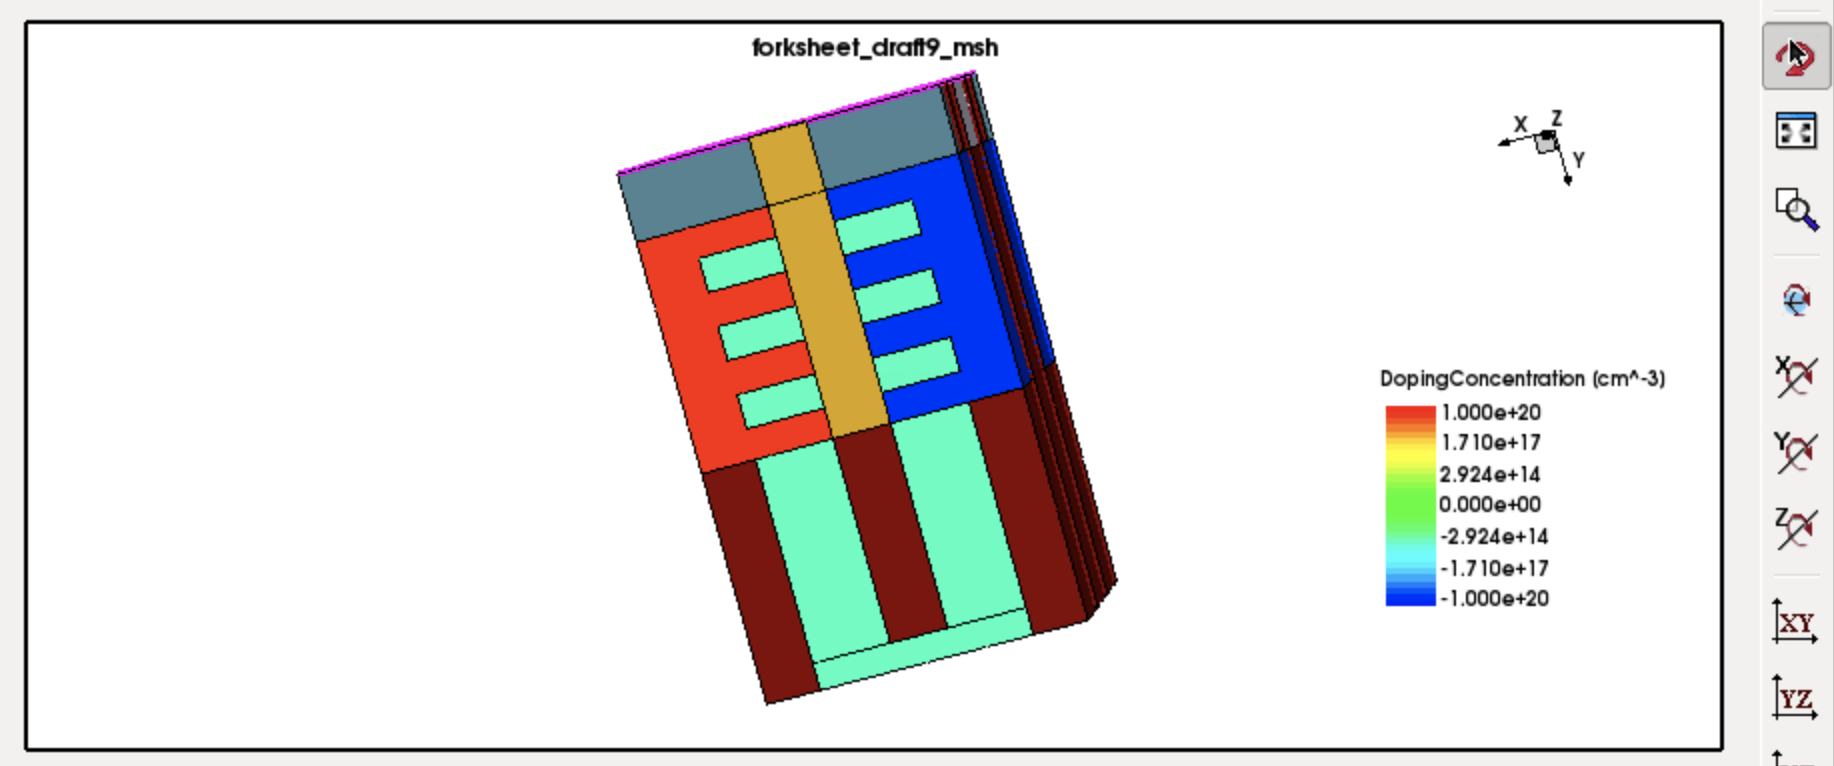
\includegraphics[width=.9\linewidth]{Screen Shot 2022-02-26 at 3.13.29 PM.png}
    \caption{Plot showing full 3D CAD structure of the FSH. Includes doping and gate contact information as well}
    \label{fig:knngraph1}
\end{figure}

\begin{figure}[H]
    \centering
    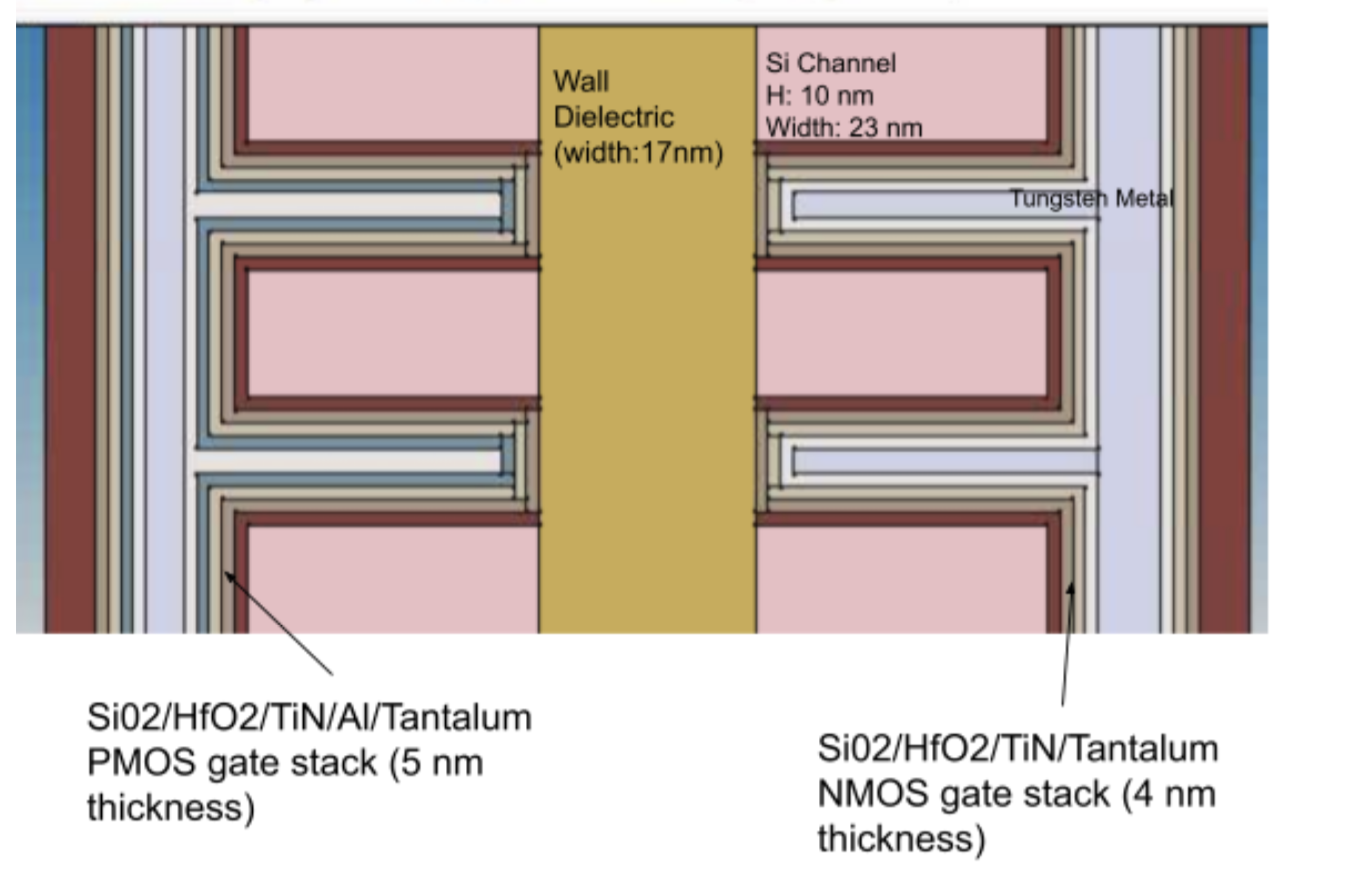
\includegraphics[width=.9\linewidth]{Screen Shot 2022-02-26 at 9.27.22 PM.png}
    \caption{Plot showing the specific gatestack for our CAD model \cite{c5}}
    \label{fig:knngraph1}
\end{figure}

\begin{figure}[H]
    \centering
    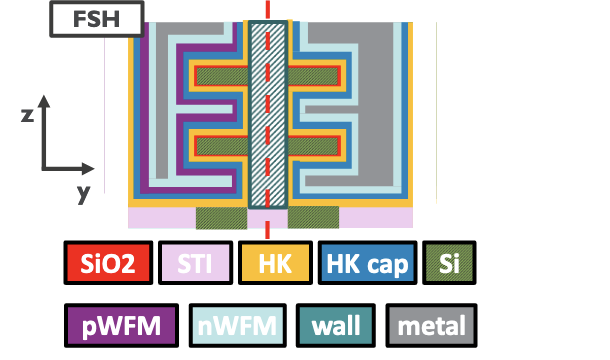
\includegraphics[width=.9\linewidth]{Screen Shot 2022-02-26 at 10.04.03 PM.png}
    \caption{State of the Art Interior of FSH as described by \cite{c6} }
    \label{fig:knngraph1}
\end{figure}


\begin{figure}[H]
    \centering
    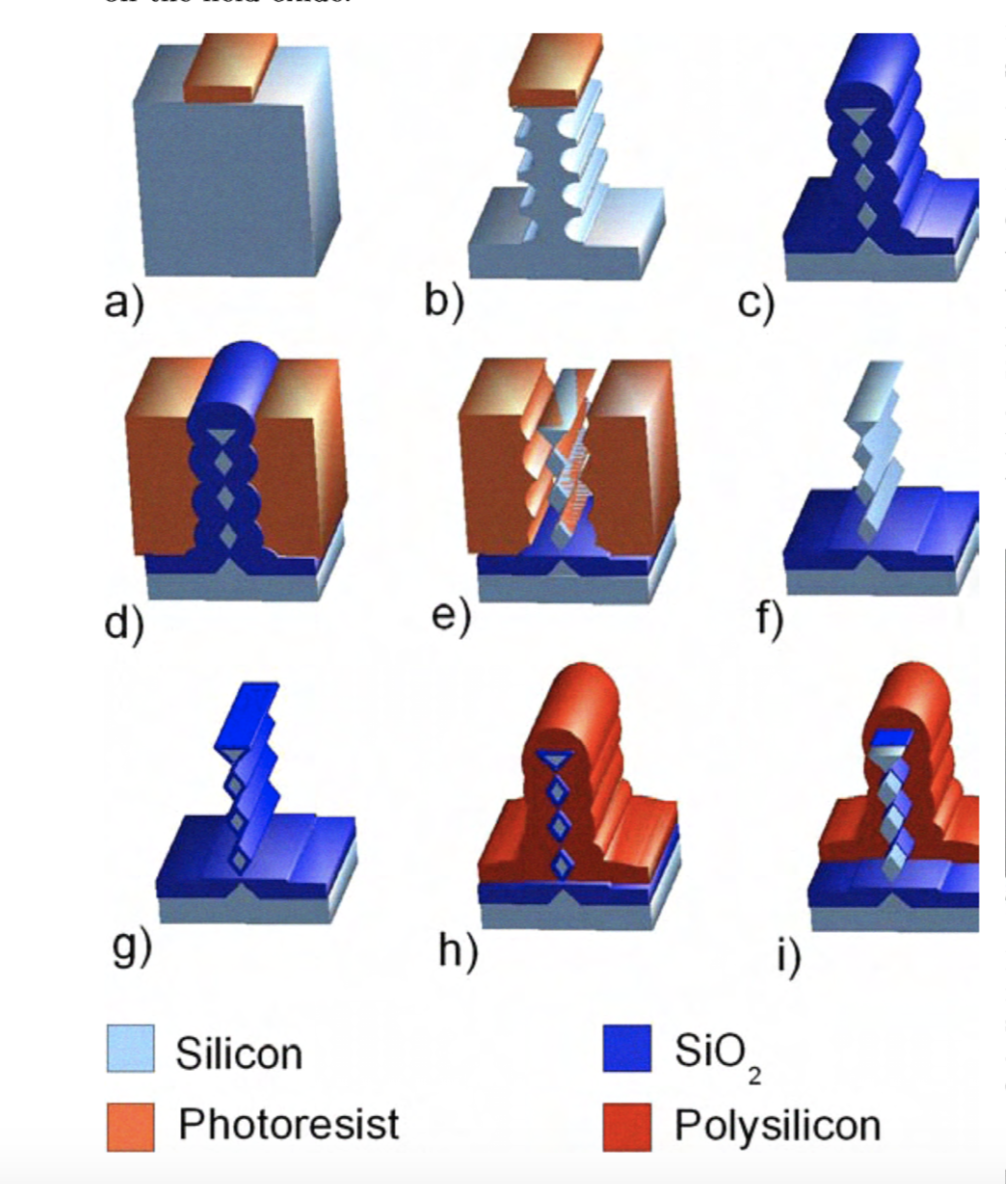
\includegraphics[width=.9\linewidth]{Screen Shot 2022-03-03 at 3.29.17 PM.png}
    \caption{Graphic showing nano-wire fabrication process}
    \label{fig:knngraph1}
\end{figure}

\begin{figure}[H]
    \centering
    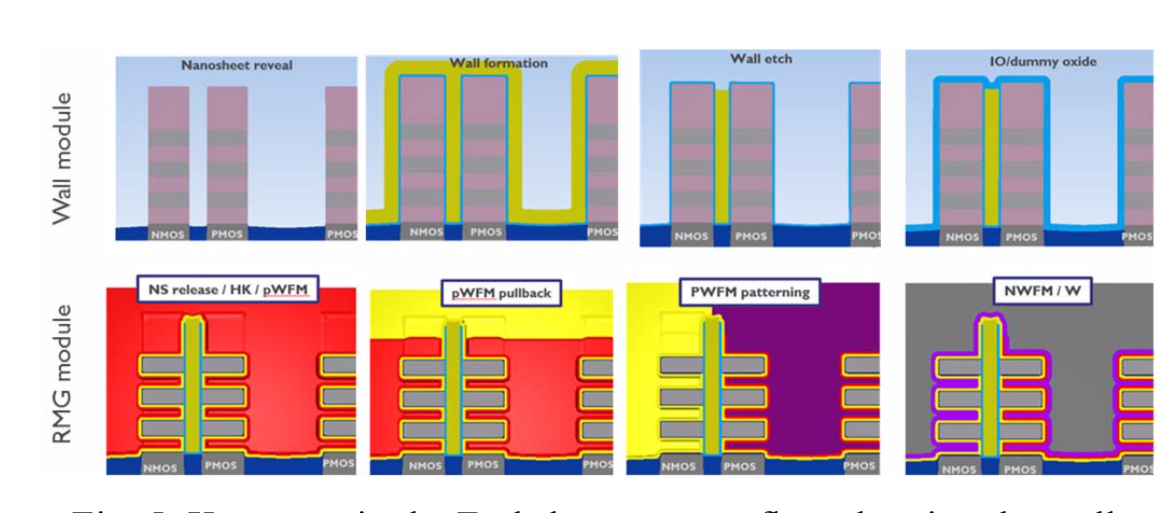
\includegraphics[width=.9\linewidth]{Screen Shot 2022-03-03 at 3.28.55 PM.png}
    \caption{Graphic showing overview of FSH fabrication process \cite{c6} }
    \label{fig:knngraph1}
\end{figure}


\begin{figure}[H]
    \centering
    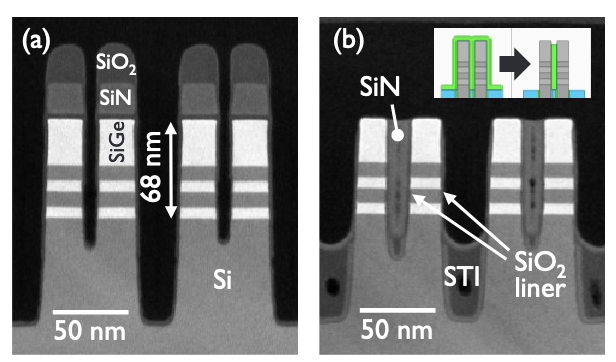
\includegraphics[width=.9\linewidth]{Screen Shot 2022-03-03 at 3.54.30 PM.png}
    \caption{TEM Image of depositing  wall dielectric \cite{c13} }
    \label{fig:knngraph1}
\end{figure}


\begin{figure}[H]
    \centering
    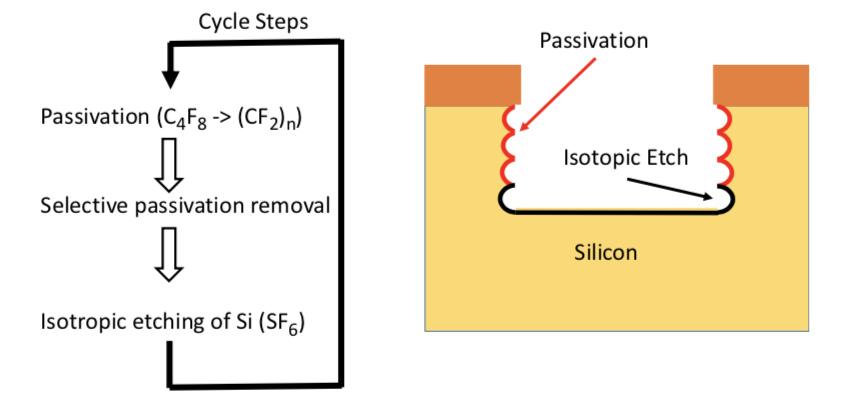
\includegraphics[width=.9\linewidth]{Screen Shot 2022-03-03 at 4.12.00 PM.png}
    \caption{Graphic showing the Bosch Process \cite{c14} }
    \label{fig:knngraph1}
\end{figure}


\begin{figure}[H]
    \centering
    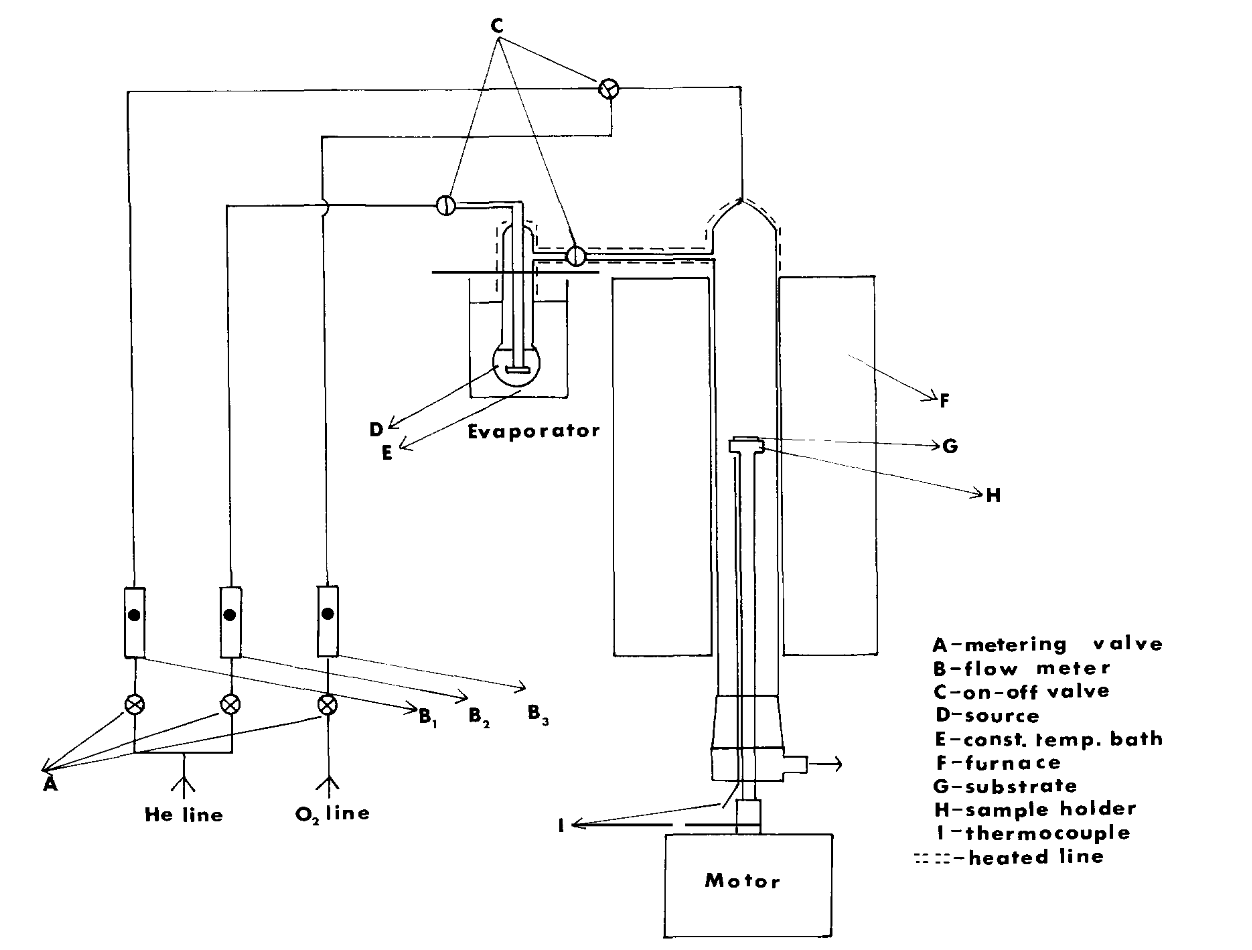
\includegraphics[width=.9\linewidth]{Screen Shot 2022-03-03 at 7.35.34 PM.png}
    \caption{Diagram showing a general CVD system \cite{c9} }
    \label{fig:knngraph1}
\end{figure}


\end{document}
